%!TEX encoding=UTF-8
\documentclass[ 4paper,11pt,openany]{book}
\usepackage[T1]{fontenc}
\usepackage[english,italian]{babel}
\usepackage{graphicx}
\usepackage[margin=1in]{geometry}


\title{Progetto Lavoratori Stagionali}

\author{Christian Farina, VR456150\\  Stefano Zenaro, VR456736}
\date{anno 2021/2022}

\begin{document}
\frontmatter
\maketitle
\tableofcontents 

\mainmatter
\chapter{Introduzione}
Riassunto del progetto
 
\chapter{Struttura del progetto}%in questa parte metteremo i vari schemi
\section{Casi d'uso principali}
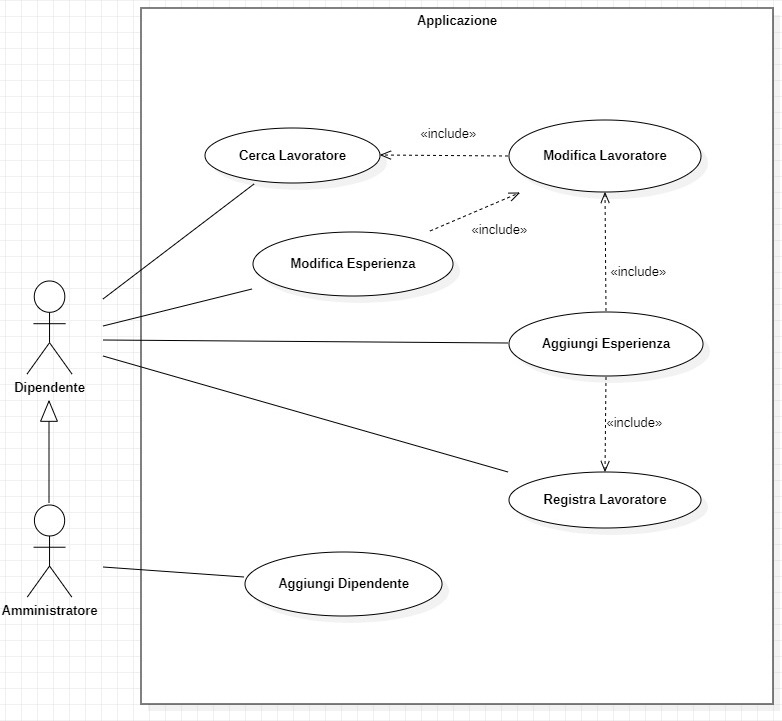
\includegraphics[width=180mm]{casi.jpg}
\section{Diagrammi di sequenza}
\subsection{Creazione e modifica di un lavoratore}
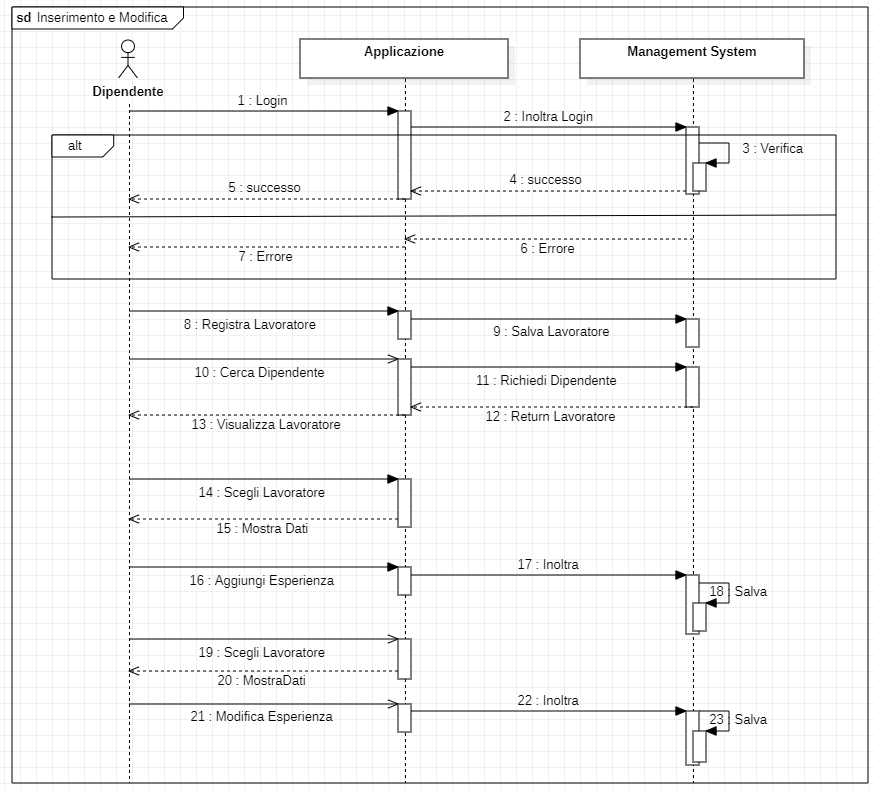
\includegraphics[width=180mm]{seq.png}
\subsection{Creazione di un dipendente}
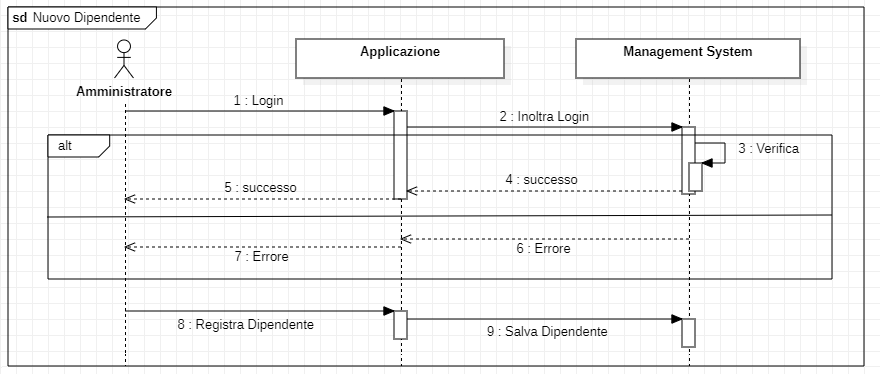
\includegraphics[width=180mm]{seq2.png}


\chapter{Implementazione}%in questa parte spiegheremo le robe di programmazione (pattern robe di progetto e minchiate varie)

\end {document}